%%%%%   INTRODUCCIÓN   %%%%%
%---------------------------------------------------------
%\section{Objetivo del documento}
%    El presente documento \varCveDocumento\ tiene como objetivo mostrar en detalle los requerimientos funcionales y no funcionales, modelos de información, reglas de negocio, modelos de comportamiento, casos de uso e interfaces correspondientes a cada uno de los módulos propuestos para esta etapa.

\section{Antecedentes}

%En la antigüedad se realizaban procedimientos que carecían de valor terapéutico y muchos de estos tratamientos mas que ayudar al paciente complicaban la situación.\\
%Fue hasta el siglo XX en que la medicina empezó a contar con un arsenal terapéutico que ya tenia una efectividad comprobada.\\
%Al día de hoy se cuenta con un mayor conocimiento de las enfermedades, de como combatirlas, de saber interpretar los síntomas y que escenarios fomentan a su desarrollo. Como es mencionado en el estudio " El tratamiento medico: Experiencia, base teórica y método " en la segunda mitad del siglo pasado se desarrollo la metodología de los ensayos clínicos aleatorios, que es hasta el momento el recurso mas confiable para conocer la efectividad real de cualquier tipo de tratamientos, aunque a pesar de la gran cantidad de ensayos clínicos realizados, mucho mas de la mitad de los tratamientos que se practican no han sido sometidos a esa prueba, lo cual no impide que sean utilizados siempre y cuando, haya un base teórica aceptable y lógica que apoye sus beneficios.\\
%La medicina es una ciencia inexacta ya que esta cuenta con el factor biológico de cada individuo es por eso que los tratamientos médicos necesitan contar un metodología que se encargara de sistematizar y ordenar los pasos que tendrán de base para tener un terapéutica racional.
%El origen de cualquier metodología medica tiene sustento en la guía propuesta en la Universidad de Groningen en Holanda y que con el apoyo de la Organización Mundial de la salud presentan 6 pasos que se espera que se acondicionen a las condiciones de trabajo.
%Cuando un profesional de la salud esta por ejecutar una prescripción medica debe de ser consciente que un tratamiento medico no debe de ser un reflejo de las quejas del paciente, ni que por cada síntoma se tendrá que prescribir un medicamento, o que dos pacientes pueden ser ajustados para llevar el mismo procedimiento clínico.\\
%Muchas veces se puede llegar a tener un prescripción inadecuada de medicamentos, del uso excesivo de medicamentos por complacencia del cliente.  
%Los pasos que se recomiendan para el profesional de la salud son los siguientes:
%\begin{itemize}
%	\item Definir el o los problemas de la salud del paciente
%	\item Especificar los objetivos del tratamiento(alcance del tratamiento)
%	\item Diseñar el esquema terapéutico mas apropiado para las necesidades del paciente
%	\item Brindar información, instrucciones y advertencias
%	\item Supervisar la evolución del tratamiento	
%\end{itemize}
%Ahora que entendemos como se realiza un prescripción medica, podemos entender a los tratamientos médicos son un conjunto de procedimientos higiénicos, farmacológicos y de rehabilitación que son recetados por un profesional de la salud para el bienestar del paciente. Por la naturaleza de los tratamientos médicos y su complejidad al administrarlo, la similitud en los múltiples medicamentos en el mercado, su poca claridad en las etiquetas, entre muchas otras cosas más conlleva a que se produzcan errores de medicación y que éstos a su vez provoquen efectos adversos a los pacientes. De acuerdo a la NCCMERP\footnote{National Coordinating Council for Medication Error Reporting and Prevention} define los errores de medicación como "cualquier incidente prevenible que puede causar daño al paciente o dar lugar a una utilización inapropiada de los medicamentos"\cite{Referencia3}. Dichos errores de medicación podrían ser solventados con el uso de las nuevas tecnologías de información.

Para la OMS (Organización Mundial de la Salud) enfermedad es la alteración o desviación del estado fisiológico en una o varias partes del cuerpo, por causas en general conocidas, manifestada por síntomas y signos característicos, y cuya evolución es más o menos previsible.\\
Para el Diccionario Médico Teide, una enfermedad se le llama al conjunto de alteraciones morfológico estructurales que se producen en organismo como consecuencia de un agente morbígeno interno o externo, contra el cual, el organismo no tiene la capacidad de oponerse o no consigue enfrentarlo con la suficiente fuerza.\\
Como podemos notar, existen diversas definiciones para el concepto de la enfermedad pero todas ellas convergen en que es una alteración o rompe la armonía del bienestar ya sea a nivel molecular, corporal, mental, emocional o espiritual.
Estas enfermedades cuentan con una amplia clasificación:
\begin{itemize}
	\item Enfermedades infecciosas: Destacadas por la presencia de bacterias, virus y hongos.
	\item Enfermedades congénitas: Adquiridas en el momento de la gestación del embrión.
	\item Enfermedades hereditarias: Su característica principal es la transmisión de generación a generación.
	\item Enfermedades auto-inmunes: El sistema inmunológico deja de reconocer ciertas células del propio organismo.
	\item Enfermedades neurodegenerativas: Desordenes cognitivos producidos por la disminución de neuronas.
	\item Enfermedades mentales: Alteraciones y trastornos cerebrales causados por desordenes químicos.
	\item Enfermedades metabólicas: Perturbaciones o alteraciones en el metabolismo
\end{itemize} 
Para poder combatir esta amplia variedad de enfermedades toman protagonismo los medicamentos que a partir de 1940 se empiezan a producir en masa.\\
Un medicamento se puede entender como toda sustancia o combinación de sustancias poseedoras de propiedades para el tratamiento, prevención de enfermedades o para el alivio de los síntomas.
Al tener un amplio espectro de enfermedades también hay una gran variedad de medicamentos, que atacan distintos problemas de diversas maneras.
Los medicamentos que se tienen son:
\begin{itemize}
	\item Analgésicos: Grupo de tipos de medicamentos en donde se encuentran todos los fármacos que tienen como finalidad aliviar el dolor físico. Estos medicamentos pueden ser divididos en dos grandes familias, los opiáceos (no esta permitida la automedicación) y los no opiáceos.
		
	\item Antiácidos y antiulcerosos: Su principal característica es la disminución de las secreciones gástricas. Si disminuye la acidez, se previene la aparición de úlceras.
	
	\item Antialérgicos: Se agrupan fármacos que tienen la finalidad de combatir los efectos negativos de las reacciones alérgicas o la hipersensibilidad.
	
	\item Antidiarreicos y laxantes: Los antidiarreicos tienen como funcionalidad detener los efectos de la diarrea. Los laxantes al contrario de los antidiarreicos su principal función es el de aumentar el movimiento intestinal.
	
	\item Antiinfecciosos: Los medicanemtos antiinfecciosos se pueden dividir en 4:
		\begin{itemize}
			\item antibiotico: Su aplicación es contra bacterias.
			\item antifúngicos: Su aplicación es contra los hongos.
			\item antivirales: Su aplicación es contra los virus.
			\item antiparasitarios: Su aplicación es contra parásitos.
		\end{itemize}
	
	\item Antiinflamatorios: Reduce la inflamación.
	
	\item Antipiréticos: Son los medicamentos encargados de bajar la fiebre.
	
	\item Antitusivos y mucolíticos: Los medicamentos antitusivos son los encargados en reducir la tos que no libre la mucosidad, al contrario los mucolíticos son los encargados de ayudar a la correcta respiración.
	 
\end{itemize}
Los medicamentos tienen que ser administrados y recomendados por un profesional de la salud, en donde te suministrará un tratamiento médico en el entendido de que un tratamiento es un conjunto de procedimientos higiénicos, farmacológicos y de rehabilitación que son recetados por un profesional de la salud para el bienestar del paciente. 

Un medicamento, según la definición propuesta por CedimCat (Centre d'Informació de Medicaments de Catalunya)\cite{Referencia1}, es una sustancia con propiedades para el tratamiento o la prevención de enfermedades en los seres humanos. También se consideran medicamentos aquellas sustancias que se utilizan o se administran con el objetivo de restaurar, corregir o modificar funciones fisiológicas del organismo o aquellas para establecer un diagnóstico médico. Estos medicamentos deben ser recetados por un Doctor y deben de ser consumidos en la forma en que se especifica en su tratamiento médico.

Un tratamiento médico es el conjunto de procedimiento higiénicos, dietéticos, farmacológicos, quirúrgicos y de rehabilitación, empleados en la atención de la salud\cite{Referencia2} cuya finalidad es la curación o el alivio de las enfermedades.

Existen varios tipos de tratamientos eficaces que se enlistan a continuación\cite{Referencia3}:
\begin{itemize}
	\item Cirugía o tratamiento quirúrgico
	\item Dieta
	\item Farmacoterapia o tratamiento con medicamentos
	\item Fisioterapia
	\item Hidroterapia
	\item Logopedia
	\item Ortopedia
	\item Prótesis: dentales, lentes, etc.
	\item Psicoterapia
	\item Quimioterapia
	\item Radioterapia
	\item Rehabilitación o tratamiento rehabilitador
	\item Reposo domiciliario
	\item Sueroterapia
	\item Terapia de quelación
	\item Terapia ocupacional
\end{itemize}

Estos tratamientos deben ser expedidos y supervisados por un médico especialista.

El médico es el profesional de la medicina que cuenta con los conocimientos y las destrezas necesarias para diagnosticar y resolver con tratamientos médicos y con procedimientos sencillos la mayoría de los padecimientos que el ser humano sufre en su vida, desde niño hasta la vejez, con acciones frecuentemente realizadas en el consultorio del médico o en la casa del enfermo\cite{Referencia4}. El médico es la persona encargada de mantener y/o mejorar la salud de sus pacientes.

El paciente designa a un individuo que es examinado medicamente o al que se administra un tratamiento\cite{Referencia5}. Es la persona que recibe atención médica cuando se encuentra en mal estado de salud o sufre síntomas de cualquier enfermedad.

En este trabajo terminal, se propone una aplicación móvil que sirva como asistente médico.

Una aplicación movil, mejor conocida como ''app", es una aplicación de software diseñada especificamente para los dispositivos móviles\cite{Referencia6}.

''Desde 2007 la tendencia del mundo entero se ha centrado alrededor de los Smartphones y sus funcionalidades. Estos pequeños dispositivos nos acompañan a todas horas y posiblemente sean con diferencia, los aparatos electrónicos que más utilizamos durante el día."\cite{Referencia7}

Hoy en día, los dispositivos móviles son mucho más utilizados que una laptop o una computadora de escritorio. Es por esto que decidimos hacer una aplicación móvil y no una aplicación web o de escritorio.

Esta aplicación móvil será desarrollada con la tecnología de \textbf{Xamarin Forms} que es una plataforma que nos permite crear Apps nativas para iOS, Mac, Android, Windows Phone, Windows 8 y más. Además nos permite utilizar solo un lenguaje de programación C\#  y  reducir tanto los perfiles como la cantidad de equipos involucrados en el desarrollo.\cite{Referencia8}

Algunas de las ventajas de la plataforma de Xamarin Forms son: 
\begin{itemize}
	\item Aplicaciones 100\% nativas
	\item Un solo lenguaje de programación que es C\#
	\item IDEs sencillos como Xamarin Studio y Visual Studio
	\item Código compartido
\end{itemize}




%\section{Contexto de trabajo}
%
%
%Se trabajara una vez que se haya terminado el marco teórico.
%
%Los seres humanos somos vulnerables a contraer distintos tipos de enfermedades por malos hábitos, por la poca actividad física, debilidades en el sistema inmunológico, entre muchas cosas más, provocando así la necesidad de acudir con un doctor que nos dará un tratamiento médico en donde con un conjunto de procedimientos higiénicos, farmacológicos, de rehabilitación y de acuerdo a las aflicciones y síntomas que presentemos se esperara curar o disminuir el impacto en nuestra salud.

\section{Objetivo}
Analizar, diseñar y desarrollar un asistente móvil que permita ayudar al usuario a llevar un mejor control de sus tratamientos médicos por medio de recordatorios y alertas que auxilien a dar un correcto seguimiento, además de notificar cuando el medicamento de dicho tratamiento esté por terminarse para que el usuario tenga la oportunidad de adquirirlo.

\section{Problemática}

La problemática a la que nos enfrentamos en este trabajo terminal es la complejidad de crear recordatorios que nos ayuden a seguir los tratamientos médicos, ya que por la complejidad de seguirlos al pie de la letra son abandonados de forma parcial o completa.\\
Carlos Baños vicepresidente para latinoamerica de los laboratorios Eli Lilly informó que cuatro de diez pacientes que se encuentran en un tratamiento médico lo abandonan de forma parcial o completa \cite{Referencia9}.\\
En consecuencia a esta mala práctica y de acuerdo con la OMS(Organización Mundial de la Salud)\cite{Referencia10} el incumplimiento en un tratamiento médico causa:
\begin{itemize}
	\item Poca o nula obtención de lo beneficios de los medicamentos.
	\item Efectos secundarios no esperados.
	\item Aumenta la probabilidad de resistencia que pueden tener las bacterias, virus, hongos o parásitos a los medicamentos recetados.
\end{itemize}
El informe se elaboró teniendo en cuenta una amplia gama de trastornos crónicos y de factores de riesgo, y buscando los puntos comunes entre ellos\cite{Referencia11}.
Las principales causas para que un paciente abandone su tratamiento de forma parcial o completa de acuerdo a un trabajo doctoral del doctor \textbf{Pablo Herrera Salinas}\cite{Referencia12} son las siguientes:
\begin{itemize}
	\item Negación a estar enfermos: Los pacientes son renuentes a la idea de estar enfermos, creyendo que solo la gente débil o vieja se enferma.
	\item Baja calidad de vida: Los pacientes creen que el seguir un tratamiento hará que su calidad de vida sea deplorable.
	\item Miedo por efectos secundarios o adicción: Los pacientes tienen miedo de los efectos secundarios que según ellos podrían ocasionar ó que se vuelvan adictos a los medicamentos.
	\item Alejarse de sus círculos sociales: Para los pacientes el seguir un tratamiento significa "obligar" a que los demás coman sin sal o que puedan ser excluidos de eventos sociales por sus restricciones.
	\item Dejar de ser independientes: A los pacientes les da miedo volverse dependientes de su tratamiento o vivir con demasiadas prohibiciones.
	\item Depresión: Los pacientes creen que no vale la pena seguir el tratamiento ya que tienen la sensación de que no sirve de nada o que es una tarea demasiado difícil.
	\item Creencias: Muchos de los pacientes por las creencias religiosas y sobre el entorno de la vida que tienen deciden no seguir al cien por ciento el tratamiento.
\end{itemize}

%La problemática a la que nos enfrentamos en este trabajo terminal es el abandono parcial o completo de los tratamientos médicos por la complejidad de seguirlos al pie de la letra y llegar a su término. Carlos Baños vicepresidente para latinoamerica de los laboratorios Eli Lilly informo que cuatro de diez pacientes que se encuentran en un tratamiento medico lo abandonan de forma parcial o completa \cite{Referencia1}.\\
%En consecuencia a esta mala practica y de acuerdo con la OMS(Organización Mundial de la Salud) el incumpliento en un tratamiento medico causa:
%\begin{itemize}
%	\item Poca o nula obtención de lo beneficios de los medicamentos.
%	\item Efectos secundarios no esperados.
%	\item Aumenta la probabilidad de resistencia que pueden tener las bacterias, virus, hongos o parásitos a los medicamentos recetados.
%\end{itemize}
%El informe se elaboró teniendo en cuenta una amplia gama de trastornos crónicos y de factores de riesgo, y buscando los puntos comunes entre ellos\cite{Referencia2}.

\section{Solución Propuesta Por Otras Aplicaciones}

En la tabla \ref{SolucionesProp} se muestran las aplicaciones que están enfocadas al ámbito de la salud y que intentan cumplir con la problemática planteada pero que ninguna de ellas cumple.

\begin{table}[H]
	\resizebox{18cm}{!} {
	
	\begin{tabular}{|l|c|c|c|c|c|c|c|}
		\hline
		\multicolumn{1}{|c|}{Aplicación} & Multiplataforma & \begin{tabular}[c]{@{}c@{}}Notificaciones\\ de\\ Medicamentos\end{tabular} & \begin{tabular}[c]{@{}c@{}}Alertas\\ a contactos\\ de Emergencia\end{tabular} & \begin{tabular}[c]{@{}c@{}}Información\\ de\\ Medicamentos\end{tabular} & \begin{tabular}[c]{@{}c@{}}Múltiples\\ perfiles\end{tabular} & \begin{tabular}[c]{@{}c@{}}Historial\\ de\\ Medicamentos\end{tabular} & \begin{tabular}[c]{@{}c@{}}Captura\\ de\\ tratamiento\end{tabular} \\ \hline
		RecuerdaMed                      & Sí              & Sí                                                                         & No                                                                            & No                                                                      & Sí                                                           & No                                                                    & Sí                                                                 \\ \hline
		Dosecast                         & Sí              & Sí                                                                         & No                                                                            & No                                                                      & No                                                           & \begin{tabular}[c]{@{}c@{}}Sí\\ (Solo Premium)\end{tabular}           & Sí                                                                 \\ \hline
		Medisafe                         & Sí              & Sí                                                                         & No                                                                            & No                                                                      & \begin{tabular}[c]{@{}c@{}}Sí\\ (Solo Premium)\end{tabular}  & No                                                                    & Sí                                                                 \\ \hline
		PillManager                      & Sí              & No                                                                         & No                                                                            & No                                                                      & No                                                           & Sí                                                                    & Sí                                                                 \\ \hline
		PharApp                          & Sí              & No                                                                         & No                                                                            & Sí                                                                      & No                                                           & No                                                                    & No                                                                 \\ \hline
		Capzule                          & Sí              & Sí                                                                         & No                                                                            & No                                                                      & No                                                           & Sí                                                                    & Sí                                                                 \\ \hline
		Andaman7                         & Sí              & No                                                                         & No                                                                            & No                                                                      & Sí                                                           & Sí                                                                    & Sí                                                                 \\ \hline
		GenieMD                          & Sí              & Sí                                                                         & No                                                                            & Sí                                                                      & Sí                                                           & No                                                                    & Sí                                                                 \\ \hline
		Rem-Pills                          & Sí              & Sí                                                                         & Sí                                                                            & Sí                                                                      & Sí                                                           & Sí                                                                    & Sí                                                                 \\ \hline
	\end{tabular}
	}
\caption{Soluciones Propuestas Por Otras Aplicaciones}
\label{SolucionesProp}
\end{table}

\begin{itemize}
	\item RecuerdaMed: Es una app que sirve como recordatorio para mejorar la cumplimentación del tratamiento sobre todo de pacientes crónicos polimedicados. Posibilita al paciente, o la persona que lo cuida, llevar un control exhaustivo de la medicación que está tomando, sin embargo, no cuenta con información de los medicamentos ni guarda el historial de los medicamentos del paciente. Es una aplicación difícil de manejar porque su interfaz no es intuitiva.

	\item Dosecast: Es una aplicación de administración de medicamentos en la cual podrá registrar su tratamiento médico para recordar tomar la medicación correcta. Esta aplicación no cuenta con alertas a contactos de emergencia, información de los medicamentos, tampoco es capaz de manejar múltiples perfiles. La aplicación si maneja un historial de medicamentos pero únicamente en su versión Premium que tiene un costo de \$59.00 pesos al mes, lo cual muchas veces es un impedimento económico para el usuario.

	\item Medisafe: Medisafe es una aplicación que ayuda a resolver el problema de incumplimiento de la medicación pero no cuenta con un servicio de alertas a contactos de emergencia ni se puede guardar la información adicional de los medicamentos. Esta aplicación cuenta con el servicio de múltiples perfiles en su versión Premium que tiene un costo de \$89.00 pesos al mes, lo cual muchas veces es un impedimento económico para el usuario.
	
	\item PillManager: Esta aplicación sirve como un recordatorio de dosificación de medicamentos pero no cuenta con un servicio de notificaciones de medicamentos para el usuario, un servicio de alertas a contactos de emergencia, no se puede guardar la información de los medicamentos y no es capaz de manejar múltiples perfiles. La interfaz de esta aplicación tiene íconos que se pueden entender fácilmente pero entre tantas opciones es fácil confundirse al querer hacer la captura de un tratamiento médico.

	\item PharApp: Es una aplicación que impulsa la adherencia del paciente al tratamiento farmacológico prescrito con independencia del tipo de medicamento y su forma de administración, sin embargo, no cuenta con un servicio de notificaciones de medicamentos para el usuario ni de alertas a los contactos de emergencia. Como esta aplicación no permite la captura del tratamiento médico, tampoco permite que se pueda generar un historial de los medicamentos del paciente. Al querer entrar a esta aplicación por primera vez, muestra un mensaje que dice que para poder hacer uso de la aplicación debemos acudir a su farmacia de confianza a pedir su usuario y contraseña, pero no explica a qué tipos de farmacia ni cuál sería el procedimiento para registrarse por lo que la mayoría de las veces, ni las farmacias tienen idea de cómo funciona esta aplicación.
	
	\item Capzule: Es una aplicación que está diseñada para seguir la salud y el bienestar de la familia, sin embargo, no se puede seguir el bienestar de la familia si no cuenta con un servicio de múltiples perfiles y de alertas a contactos de emergencia. La interfaz de esta aplicación no es nada intuitiva y es difícil entender su funcionamiento.

	\item Andaman7: Es una aplicación que facilita la administración de sus datos de salud por medio de la captura del tratamiento. La desventaja de esta aplicación es que no cuenta con notificaciones al usuario ni alertas a sus contactos de emergencia. 
	
	\item GenieMD: Es la primer plataforma de telemedicina totalmente funcional, basada en la nube y móvil. Algunas de las desventajas de esta aplicación es que no maneja alertas a contactos de emergencia, no puede generar un historial de medicamentos y tiene una interfaz un poco difícil de entender.
	
\end{itemize}

	
\section{Solución Propuesta}
Como podemos notar ninguna aplicación existente en el mercado da solución a la problemática planteada.
Es por eso que en este trabajo terminal se propone una aplicación móvil que llamaremos \textbf{Rem-Pills} y su principal objetivo es facilitar la creación de los recordatorios para la ayuda del seguimiento de los tratamientos médicos.\\
Para poder cumplir nuestro objetivo se proponen las siguientes características:
\begin{itemize}
	\item Multiplataforma para iOs y Android.
	
	\item Una interfaz intuitiva que ayude a mejorar los niveles de usabilidad en los usuarios en el momento en que agreguen sus tratamientos médicos.
	
	\item Programación de recordatorios los cuales contarán con notificaciones audiovisuales.
	
	\item Alertas a los contactos de emergencia que serán activadas cuando un recordatorio no sea finalizado después de 3 avisos.
	
	\item Información acerca de la utilización, efectos secundarios y principales usos de los medicamentos.
	
	\item Historial semanal, mensual o anual de los medicamentos, tratamientos clínicos y datos relevantes de la salud del usuario.
	
\end{itemize}



%Por lo visto en la sección anterior, en este trabajo terminal se propone una aplicación móvil llamada Rem-Pills que tiene como principal objetivo cumplir con la problemática y para poder cumplir con esta se proponen las siguientes características.
%\begin{itemize}
%	\item Multiplataforma para Android y iOS.
%	
%	\item Una interfaz intuitiva que ayude a mejorar los niveles de usabilidad en los usuarios en el momento en que agreguen sus tratamientos medicos.
%
%	\item Programación de recordatorios los cuales contaran con notificaciones audiovisuales.
%	
%	\item Múltiples perfiles.
%	
%	\item Alertas a los contactos de emergencia que serán activadas cuando una notificación no sea silenciada después de 3 avisos.
%	
%	\item Información acerca de la utilización, efectos secundarios y principales usos de los medicamentos.
%	
%	\item Historial semanal, mensual o anual de los medicamentos, tratamientos clinicos y datos relevantes de la salud del usuario.
%	
%\end{itemize}

\section{Análisis de factibilidad}
\subsection{Económica}

Este estudio tiene como finalidad determinar la factibilidad económica y observar el total de los gastos que generan los recursos que son necesarios para el desarrollo del trabajo terminal \textbf{ Asistente Móvil para el Seguimiento de Tratamientos Médicos Rem-Pills}, cabe mencionar que es un proyecto únicamente con fines académicos y sin fines de lucro.\\

Los gastos que generaron los recursos necesarios para el desarrollo de este proyecto podemos clasificarlos de la siguiente manera:

\begin{enumerate}
	\item Gastos Tecnológicos
	\item Gastos de Servicios
	\item Sueldos
\end{enumerate}

A continuación se describen cada uno de los gastos anteriormente mencionados y los recursos que los comprenden.

\subsubsection{Gastos Tecnológicos}
Los gastos tecnológicos son aquellos que se generan con los recursos de hardware utilizados durante el desarrollo de este proyecto.\\
Los recursos de hardware son considerados como un activo fijo y por lo tanto, sufren una depreciación técnica. La depreciación es la disminución en el valor de mercado de un bien, la disminución en el valor de un activo para su propietario, o la asignación del costo de uso o demerito de un activo a lo largo de su vida útil (duración)\cite{Referencia15}.\\\\

En la siguiente tabla \ref{GastosTecnologicos} se muestra el hardware disponible para el desarrollo de este trabajo terminal y el gasto total del mismo en un periodo de \textbf{10 meses} que es el tiempo en que se estará desarrollando este proyecto.

\begin{table}[H]
	\centering
	\resizebox{13cm}{!} {
	\begin{tabular}{|c|c|c|c|c|}
	\hline
	\multicolumn{1}{|c|}{Recurso} & Precio & \begin{tabular}[c]{@{}c@{}}Valor\\ de\\ Salvamento\end{tabular} & \begin{tabular}[c]{@{}c@{}}Depreciación\\ mensual\end{tabular} & \begin{tabular}[c]{@{}c@{}}Depreciación\\ total\end{tabular}\\ \hline
	Macbook Pro 13 2011 & \$12,000.00  & \$3,600.00  & \$140.00 & \$1,400.00 \\ \hline
	Gateway  NE 522 series & \$4,500.00  & \$1,350.00 & \$52.50   & \$525.00  \\ \hline
Total  &  &   &  & \$1,925.00 \\ \hline
                                                       
\end{tabular}
}
\caption{Gastos Tecnológicos}
\label{GastosTecnologicos}
\end{table}

\subsubsection{Gastos de Servicios}
Este trabajo terminal también conlleva gastos de servicios públicos necesarios para el desarrollo del proyecto como lo son el servicio de internet y el servicio de electricidad necesario para la funcionalidad de los equipos de cómputo utilizados.

En la siguiente tabla \ref{GastosServicios} se muestran los gastos de servicios estimados durante el desarrollo del trabajo terminal que será durante un periodo de \textbf{10 meses}.

\begin{table}[H]
	\centering
	\resizebox{10cm}{!} {
		\begin{tabular}{|c|c|c|}
			\hline
			\multicolumn{1}{|c|}{Recurso} & Gasto mensual & Gasto total\\ \hline
			Electricidad & \$133.00  & \$1,330.00 \\ \hline
			Internet & \$166.00  & \$1,660.00 \\ \hline
			Total  & \$360.00 & \$2,990.00 \\ \hline
			
		\end{tabular}
	}
	\caption{Gastos de Servicios}
	\label{GastosServicios}
\end{table} 

\subsubsection{Sueldos}
Los gastos de sueldos son los gastos relacionados con los sueldos del personal necesario para el desarrollo de este proyecto. Para el desarrollo del trabajo terminal se han considerado un análista, un desarrollador y un tester, de los cuales se muestra en la siguiente tabla \ref{Sueldos} el tiempo de trabajo y sus sueldos estimados por hora para el Trabajo Terminal 1.

\begin{table}[H]
	\centering
	\resizebox{14cm}{!} {
		\begin{tabular}{|c|c|c|c|c|c|}
			\hline
			\multicolumn{1}{|c|}{TT} & Recurso & \begin{tabular}[c]{@{}c@{}}Tiempo\\(meses) \end{tabular} & 
			\begin{tabular}[c]{@{}c@{}}Días\\ trabajados \end{tabular} & \begin{tabular}[c]{@{}c@{}}Tiempo\\ estimado \end{tabular} & \begin{tabular}[c]{@{}c@{}}Pago por\\ hora \end{tabular}\\ \hline
			TT1 & Analista & 3 meses  & 60 días & 240 hrs & \$140.00\\ \hline
			TT1 & Desarrollador & 1 1/2 mes  & 30 días &  120 hrs & \$130.00 \\ \hline
			TT1 & Tester  & 1/2 mes & 10 días & 40 hrs & \$85.00 \\ \hline
		    Total &	  & 5 meses & 100 días  & 400 hrs &  \\ \hline
			
		\end{tabular}
	}
	\caption{Sueldos y Tiempos para el Trabajo Terminal 1}
	\label{Sueldos}
\end{table} 

En la siguiente tabla \ref{Sueldos2} se muestra el tiempo de trabajo y sus sueldos estimados por hora para el Trabajo Terminal 2.

\begin{table}[H]
	\centering
	\resizebox{14cm}{!} {
		\begin{tabular}{|c|c|c|c|c|c|}
			\hline
			\multicolumn{1}{|c|}{TT} & Recurso & \begin{tabular}[c]{@{}c@{}}Tiempo\\(meses) \end{tabular} & 
			\begin{tabular}[c]{@{}c@{}}Días\\ trabajados \end{tabular} & \begin{tabular}[c]{@{}c@{}}Tiempo\\ estimado \end{tabular} & \begin{tabular}[c]{@{}c@{}}Pago por\\ hora \end{tabular}\\ \hline
			TT2 & Analista & 1 mes  & 20 días & 80 hrs & \$140.00\\ \hline
			TT2 & Desarrollador & 3 1/2 meses  & 70 días &  280 hrs & \$130.00 \\ \hline
			TT2 & Tester  & 1/2 mes & 10 días & 40 hrs & \$85.00 \\ \hline
			Total &	  & 5 meses & 100 días  & 400 hrs &  \\ \hline
			
		\end{tabular}
	}
	\caption{Sueldos y Tiempos para el Trabajo Terminal 2}
	\label{Sueldos2}
\end{table} 

Igualmente, durante los \textbf{10 meses} del desarrollo de este proyecto, se ha considerado la colaboración de un project manager. En la tabla \ref{pm} se muestra el tiempo de trabajo del project manager y su sueldo estimado por hora.

\begin{table}[H]
	\centering
	\resizebox{14cm}{!} {
		\begin{tabular}{|c|c|c|c|c|c|}
			\hline
			\multicolumn{1}{|c|}{TT} & Recurso & \begin{tabular}[c]{@{}c@{}}Tiempo\\(meses) \end{tabular} & 
			\begin{tabular}[c]{@{}c@{}}Días\\ trabajados \end{tabular} & \begin{tabular}[c]{@{}c@{}}Tiempo\\ estimado \end{tabular} & \begin{tabular}[c]{@{}c@{}}Pago por\\ hora \end{tabular}\\ \hline
			TT1 & Project Manager & 5 meses  & 100 días & 400 hrs & \$150.00\\ \hline
			TT2 & Project Manager & 5 meses  & 100 días &  400 hrs & \$150.00 \\ \hline
			Total &	  & 10 meses & 200 días  & 800 hrs &  \\ \hline
			
		\end{tabular}
	}
	\caption{Sueldos y Tiempos para el Project Manager}
	\label{pm}
\end{table} 

En la siguiente tabla \ref{Sueldostotales} se muestran los gastos totales por el desarrollo de este trabajo terminal.

\begin{table}[H]
	\centering
	\resizebox{14cm}{!} {
		\begin{tabular}{|c|c|c|c|}
			\hline
			\multicolumn{1}{|c|}{Cantidad} & Recurso & \begin{tabular}[c]{@{}c@{}}Tiempo\\estimado \end{tabular} & 
			\begin{tabular}[c]{@{}c@{}}Pago\\ total \end{tabular}\\ \hline
			1 & Análista & 320 hrs  & \$44,800.00 \\ \hline
			1 & Desarrollador &  400 hrs & \$52,000.00 \\ \hline
			1 & Tester & 80 hrs  & \$6,800.00 \\ \hline
			1 & Project Manager & 800 hrs  & \$120,000.00 \\ \hline
			Total &	  &  & \$223,600.00  \\ \hline
			
		\end{tabular}
	}
	\caption{Sueldos y Tiempos Totales del Trabajo Terminal}
	\label{Sueldostotales}
\end{table}

En la tabla \ref{Gastostotales} se muestra el total de los gastos tecnológicos, gastos de servicios y sueldos, necesarios para el desarrollo de este proyecto.

\begin{table}[H]
	\centering
	\resizebox{10cm}{!} {
		\begin{tabular}{|c|c|}
			\hline
			Concepto & Precio \\ \hline
			Gastos tecnológicos & \$1,925.00 \\ \hline
			Gastos de servicios& \$2,990.00 \\ \hline
			Sueldos &  \$223,600.00 \\ \hline
			Total & \$228,515.00 \\ \hline
		\end{tabular}
	}
	\caption{Gastos Totales del Trabajo Terminal}
	\label{Gastostotales}
\end{table}

Por lo tanto, el costo total estimado de este proyecto es de \$228,515.00. Y concluyendo con este análisis de factibilidad económica, se determinó que se cuenta con la infraestructura necesaria para el desarrollo de este Trabajo Terminal.

 


%\section{Referencias}
%
%\begin{thebibliography}{X}
%	
%	\bibitem{Referencia1} \textsc{CedimCat (Centre d'Informació de Medicaments de Catalunya)} \textit{CONCEPTO DE MEDICAMENTO} \textit{http://www.cedimcat.info/index.php?option=com\_content\&view=article\&id=209:que-es-un-medicamento\&catid=40\&Itemid=472\&lang=es} \textsc{July 2016}
%	
%	\bibitem{Referencia2} \textsc{La Comisión Nacional de Arbitraje Médico} \textit{GLOSARIO DE TÉRMINOS MÉDICO-JURÍDICOS} \textit{http://www.conamed.gob.mx/comisiones\_estatales/coesamed\_nayarit/publicaciones/pdf/glosario.pdf}
%	
%	\bibitem{Referencia3} \textsc{Agencia Española de Medicamentos y Productos Sanitarios.} \textit{GUÍA DE PRESCRIPCIÓN TERAPÉUTICA} \textit{Barcelona: Pharma} \textsc{2016}
%	
%	\bibitem{Referencia4} \textsc{P.S. Raymundo} y \textsc{R.S. Octavio}, \textit{SEMINARIO: EL EJERCICIO ACTUAL DE LA MEDICINA}
%	\textit{http://www.facmed.unam.mx/sms/seam2k1/2001/ponencia\_may\_2k1.htm}, EL PAPEL DE LA MEDICINA GENERAL EN EL SISTEMA NACIONAL DE SALUD
%	
%	\bibitem{Referencia5} \textsc{CommentCaMarche.net} \textit{CONCEPTO DE PACIENTE} \textit{https://salud.ccm.net/faq/15489-paciente-definicion}
%	
%	\bibitem{Referencia6} \textsc{eumed.net Enciclopedia virtual} \textit{CONCEPTO DE APLICACIÓN MÓVIL} \textit{http://www.eumed.net/libros-gratis/2016/1539/aplicacion.htm}
%	
%	\bibitem{Referencia7} \textsc{Abalit Technologies} \textit{¿Qué impacto social tienen las aplicaciones móviles?} \textit{https://www.abalit.org/blog/post/impacto-social-apps/es}
%	
%	\bibitem{Referencia8} \textsc{Marc Rubiño} \textit{Xamarin Forms uno para todos !!!} \textit{https://mrubino.net/2014/09/24/xamarin-forms-uno-para-todos/}
%	
%	\bibitem{Referencia9} \textsc{Rafael M} y \textsc{H.D. Sherali},
%	\textit{http://www.milenio.com/ciencia-y-salud/mexico-4-10-abandonan-tratamiento-eli-lilly},  En México, 4 de cada 10 abandonan su tratamiento: Eli Lilly. 12.07.2017.
%	
%	\bibitem{Referencia10} \textsc{Organización Mundial de la Salud} \textit{Adherence to Long-Term Therapies. Evidence for Action} \textit{http://www.who.int/mediacentre/news/releases/2003/pr54/es/} \textsc{July 2003}
%	
%	\bibitem{Referencia11} \textsc{Derek Yach} \textit{ADHERENCE TO LONG-TERM THERAPIES-Evidence for action
%} \textsc{January 2003}
%	
%	\bibitem{Referencia12} \textsc{Pablo Herrera Salinas . (2015)} \textsc{. ¿POR QUÉ NO SEGUIMOS LOS TRATAMIENTOS MÉDICOS E INDICACIONES DE SALUD?. 2018, de CERES DESARROLLO HUMANOY LA SECCIÓN EN ESPAÑOL DEL BRITISH GESTALT JOURNAL Sitio web:} \textit{https://www.britishgestaltjournal.com/features/2015/1/19/por-qu-no-seguimos-los-tratamientos-mdicos-e-indicaciones-de-salud}
%
%	\bibitem{Referencia13} \textsc{Generacion Googleinstein} \textit{CONCEPTO DE DEPRECIACIÓN} \textit{http://financierosudl.blogspot.com/2009/04/concepto-de-depreciacion.html} \textsc{June 2018}
%	
%	\bibitem{Referencia14} \textsc{Nativos Digitales} \textit{CONOCIENDO LA METODOLOGÍA SCRUM: SUS BENEFICIOS Y CARACTERÍSTICAS} \textit{https://nativosdigitales.pe/blog/metodologia-scrum-beneficios-caracteristicas} \textsc{March 2017}
%	
%	
%	
%	\bibitem{Referencia15} \textsc{Proyectos Agiles.org} \textit{Qué es SCRUM} \textit{https://proyectosagiles.org/que-es-scrum/} 
%	
%	 
%	
%	 
%\end{thebibliography}
%En la figura \ref{label} se muestra el diagrama de la propuesta de solución

%Por lo visto anteriormente se propone una aplicacion movil llamada Rem-Pills, que tiene como principal objetivo satisfacer la problematica planteada
%
%Por todo lo anterior se propone una aplicacion movil que llamaremos Rem-Pills, para la ayuda en el segu medicos que se 

%\section{Solución propuesta}
%Eso se encuentra en la introducción. ¿Lo dividimos o quitamos esta sección?
%
%\section{Justificación}
%
%
%\section{Objetivos}
%\subsection{Objetivo general}
%
%\subsection{Objetivos específicos}
%	\begin{itemize}
%		\item 
%	\end{itemize}	
%
%%\section{Productos o resultados esperados}
%%\textbf{Esta sección está en el protocolo pero no nos la dijo el profesor. ¿La dejamos?}
%%
%%En la Figura \ref{fig:IntroduccionArqui} se muestra la arquitectura del sistema, la cual se conforma de cuatro etapas las cuales se describen a continuación:
%
%%\begin{enumerate}
%%	\item \textbf{Sensores.} En esta etapa se tomarán las mediciones de los signos vitales  con los sensores determinados durante el análisis.
%%	\item \textbf{Digitalización.} Una vez obtenidas las mediciones de los sensores, éstas pasarán a ser digitalizadas mediante un dispositivo digital programable para obtener la señal procesada.
%%	\item \textbf{Envío de datos.} Con los datos obtenidos en la etapa anterior, se realizará el envío a un teléfono celular.
%%	\item \textbf{Recepción de datos.}  Las señales procesadas de los signos vitales serán recibidas en el teléfono celular en donde se guardará el historial de los datos para futuras consultas.
%%\end{enumerate}
%%
%%De la realización de este Trabajo Terminal se obtendrán los siguientes productos:
%%
%%\begin{enumerate}
%%	\item Código.
%%	\item Sistema embebido.
%%	\item Aplicación móvil.
%%	\item Documentación técnica del sistema.
%%	\item Manual de usuario.
%%\end{enumerate}
%%
%%\begin{figure}[htbp!]
%%	\centering
%%	\fbox{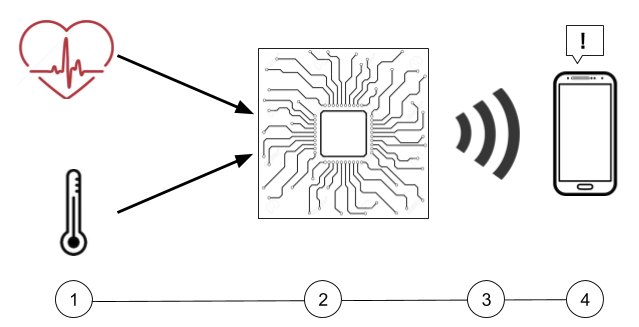
\includegraphics[width=0.8\textwidth]{images/introduccion/arquitectura.png}}
%%	\caption{Arquitectura del sistema.}
%%	\label{fig:IntroduccionArqui}
%%\end{figure}
%
%\section{Metodología}
%%Para la realización del trabajo terminal se propone emplear el Modelo en V ya que ofrece una visión detallada de los diversos pasos e interacciones relacionados con el proceso de desarrollo y puede considerarse como un flujo de trabajo comúnmente utilizado. En la Figura \ref{fig:IntroduccionMetodologia} se muestran las principales actividades abordadas por el método. Convencionalmente, el lado izquierdo del modelo representa las fases del diseño del sistema, mientras que el lado derecho representa las fases de validación y verificación del sistema integrado.
%%
%%\TODO \textbf{Cambiar resolución de imagen.}
%%\begin{figure}[htbp!]
%%	\centering
%%	\fbox{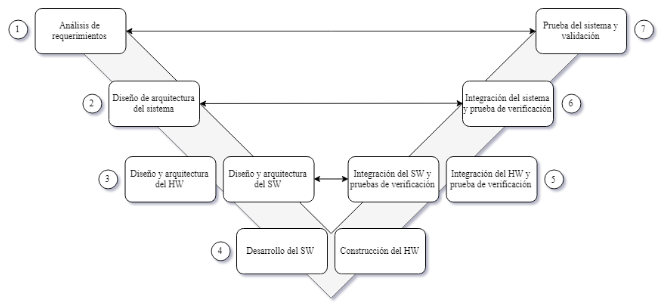
\includegraphics[width=\textwidth]{images/introduccion/metodologia.png}}
%%	\caption{Fases del modelo en V.}
%%	\label{fig:IntroduccionMetodologia}
%%\end{figure}
%%
%%El desarrollo se llevará a cabo en las siguientes etapas:
%%
%%\begin{enumerate}
%%	\item Análisis de requerimientos. Esta fase consiste en establecer qué debe hacer el sistema ideal, sin determinar cómo se construirá o diseñará el software. 
%%	\item Diseño de arquitectura del sistema. El diseño de la arquitectura del sistema consiste en varios pasos, como refinar las funciones del sistema y asignarlas a los diferentes componentes del sistema que pueden ser físicos o de hardware.
%%	\item Diseño de arquitectura de SW y HW. En esta fase del desarrollo del sistema, se diseña el hardware y el software de los diversos elementos que constituyen los componentes del sistema global. Las actividades que se aplican son similares a las realizadas en la fase anterior, pero centrándose en un componente específico del sistema: 
%%		\begin{itemize}
%%			\item Refinamiento de los requerimientos funcionales y no funcionales del hardware y software.
%%			\item Asignación de las funciones del software a los componentes de hardware.
%%		\end{itemize}
%%	\item Desarrollo del SW y Construcción del HW. Una vez que todos los componentes del sistema están diseñados, los elementos de hardware se construyen físicamente y los módulos de software son desarrollados en paralelo, y finalmente integrados con el hardware. Al final de este paso, los elementos de software y hardware deben estar disponibles para las actividades de verificación. Pueden realizarse algunas pruebas unitarias en paralelo con la implementación.
%%	\item Integración y verificación del SW y HW. En este paso se ensamblan los componentes de hardware y software. Las pruebas de verificación se ejecutan para comprobar el cumplimieno de los objetivos de diseño.
%%	\item Integración del sistema y prueba de verificación. En este paso, los elementos del sistema (HW, SW) se combinan y tiene lugar la verificación de los requisitos del sistema. 
%%	\item Prueba del sistema y validación. Esta última de verificación tiene como objetivo validar si los resultados obtenidos cumplen con los requerimientos.
%%\end{enumerate}
%
%%\section{Estructura del documento}
%%	\textbf{Creo que estaría bien agregar la descripción de los capítulos que abarca el documento pero no sé si aquí esté bien.